\documentclass[a4paper,12pt]{article} % тип документа

% Поля страниц
\usepackage[left=2.5cm,right=2.5cm, top=2cm,bottom=2cm,bindingoffset=0cm]{geometry}
    
%Пакет дял таблиц   
\usepackage{multirow} 
    
%Отступ после заголовка    
\usepackage{indentfirst}


% Рисунки
\usepackage{subcaption,floatrow,graphicx,calc}
\usepackage{wrapfig}

% Создаёем новый разделитель
\DeclareFloatSeparators{mysep}{\hspace{1cm}}

% Ссылки?
\usepackage{hyperref}
\usepackage[rgb]{xcolor}
\hypersetup{				% Гиперссылки
    colorlinks=true,       	% false: ссылки в рамках
	urlcolor=blue          % на URL
}


%  Русский язык
\usepackage[T2A]{fontenc}			% кодировка
\usepackage[utf8]{inputenc}			% кодировка исходного текста
\usepackage[english,russian]{babel}	% локализация и переносы


% Математика
\usepackage{amsmath,amsfonts,amssymb,amsthm,mathtools, mathrsfs, wasysym}

\usepackage{fancyhdr}
\pagestyle{fancy}

\begin{document}

\begin{titlepage}

\begin{center}
%\vspace*{1cm}
\large\textbf{Московский Физико-Технический Институт}\\
\large\textbf{(государственный университет)}
\vfill
\line(1,0){430}\\[1mm]
\huge\textbf{Работа 5.1.2}\\
\line(1,0){430}\\[1mm]
\vfill
\large Сибгатуллин Булат, ФРКТ\\
\end{center}

\end{titlepage}
\fancyhead[L] {Работа 5.1.3}
\noindent \textbf{Цель работы: } \\
\indent получить ВАХ эффекта на экране ЭО; измерить расстояние между характерными точками в вольтах; снять ВАХ в статическом режиме; по результатам измерений рассчитать размер электронной оболочки атома, оценить глубину потенциальной ямы и потенциал ионизации атома, заполняющего лампу.

\section{Теоретическая часть}
	К. Рамзауэр исследовал зависимость поперечных сечений упрогого рассеяния электронов (с энергией до 10 ЭВ) на атомах аргона. В результате этих исследований было обнаружено явление, получившее название \textit{эффекта Рамзауэра}.
	
	С точки зрения квантовой теории атом по отношению к электронной волне ведет себя как преломляющая среда с относительным показателем преломления
	\begin{equation*}
		n = \frac{\lambda}{\lambda^\prime} = \sqrt{1-\frac{U}{E}},
	\end{equation*}
	где $U$, $E$ -- соответственно потенциальная и полная энергии электрона внутри атома.
	
	Будем считать, что электрон рассеивается на одномерной прямоугольной потенциальной яме конечной глубины. Такая модель является хорошим приближением для атомов тяжелых инертных газов, отличающихся наиболее компактной структурой и резкой внешней границей. Решение задачи о прохождении частицы с энергией $E$ над потенциальной ямой шириной $l$ и глубиной $U_0$ не составит труда найти из уравнения Шредингера:\\
	\begin{equation*}
		\psi^{\prime\prime}+k^2\psi=0, \ \text{где}\
		k^2 =\begin{cases}
			2mE/\hbar^2 & x<0, x>l\\
			(2mE+U_0)/\hbar^2 & 0<x<l
		\end{cases}.
	\end{equation*}
	Коэффициент прохождения равен отношению квадратов амплитуд прошедшей и падающей волн и определяется выражением:
	\begin{equation*}
		\frac{1}{D} = 1 + \frac{U_0^2}{4E(E+U_0)}\sin^2(k_2l).
	\end{equation*}
	Минимум последнего выражения отвечает квантовому аналогу просветления оптики, так как при выполнении условия
	\begin{equation*}
		\tag{$\star$}
		\label{eq:uslovie}
		\sqrt{\frac{2m(E+U_0)}{\hbar^2}}l = \pi n, \ n\in\mathbb{N},
	\end{equation*}
	коэффициент прохождения частицы над ямой становится равным единице, то есть достигает своего максимального значения.
	Отметим, что условие~(\ref{eq:uslovie}) легко получить, рассматривая интерференцию электронов волн де Бройля в атоме:\\
	\begin{itemize}
		\item
			Условие первого интерференционного максимума:
			\begin{equation}
				\label{eq:1}
				2l = \frac{h}{\sqrt{2m(E_1+U_0)}}.
			\end{equation}
		\item
			Условие первого интерференционного минимума:
			\begin{equation}
				\label{eq:2}
				2l =\frac{3}{2} \frac{h}{\sqrt{2m(E_1+U_0)}}.
			\end{equation}			
	\end{itemize}

	Решая совместно уравнения~(\ref{eq:1}, \ref{eq:2}) можно получить:
	\begin{equation}
		\label{eq:l}
		l = \frac{h\sqrt{5}}{\sqrt{32m(E_2-E_1)}}.
	\end{equation}
	Понятно, что энергии $E_1$ и $E_2$ соответствуют энергиям электронов, прошедших разность потенциалов $V_1$ и $V_2$, то есть $E_1 = eV_1$ и $E_2 = eV_2$. 
	
	По измеренным величинам $E_1$ и $E_2$, используя формулы~(\ref{eq:1}, \ref{eq:2}), можно рассчитать эффективную глубину потенциальной ямы атома:
	\begin{equation}
		\label{eq:U_0}
		U_0 = \frac{4}{5}E_2 - \frac{9}{5}E_1
	\end{equation}

	Согласно квантовой механике зависимость вероятности рассеяния электрона от его энергии можно определить из соотношения:
	\begin{equation}
		\label{eq:w}
		w(U) = -\frac{1}{C}\ln \frac{I(U)}{I_0},
	\end{equation}
	где $I_0$ -- ток катода, а $C$ -- некторая постоянная.
	
	



\section{Экспериментальная установка}
	В нашей работе для изучения эффекта Рамзауэра используется тиратрон ТГ3-01/1.3Б, заполненный инертным газом. Схематическое изображение тиратрона и его конструкция приведены на рис.~\ref{pic1}.
	
	Принципиальная схема установки для изучения эффекта Рамзауэра приведена на рис.~\ref{pic2}. На лампу Л подаётся синусоидальное напряжение частоты 50 Гц от источника питания ИП, С -- стабилизированный блок накала катода; исследуемый сигнал подаётся на электронный осциллограф (ЭО); цифрами обозначены номера ножек лампы.
	
	\thisfloatsetup{floatrowsep=mysep}	
	\begin{figure}[h!]
		\ffigbox{
			\begin{subfloatrow}[2]
				\ffigbox[\FBwidth]{\caption{}}%
				{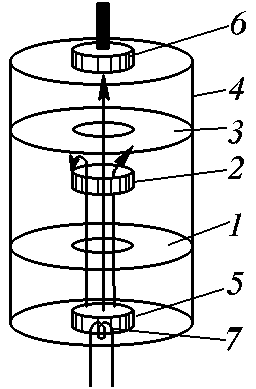
\includegraphics[width=3cm,height=4.5cm]{pic1}{\label{pic1}}}
				\ffigbox[\FBwidth]{\caption{}}%
				{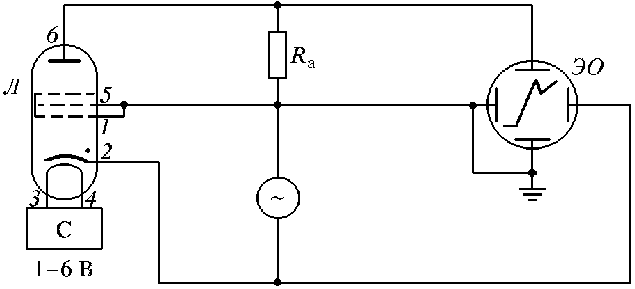
\includegraphics[width=7cm,height=4cm]{pic2}{\label{pic2}}}         
			\end{subfloatrow}
		}
		{\caption{Экспериментальная установка.}}
	\end{figure}
	
	Схема экспериментальной установки, изображённая на рис.~\ref{pic2} в нашей работе конструктивно осуществлена следующим образом. Лампа-тиратрон ТГ3-01/1.3Б, заполненная инертным газом, расположена непосредственно на корпусе блока источника питания (БИП). Напряжение к электродам лампы подаётся от источников питания, находящихся в корпусе прибора. Регулировка напряжения и выбор режима работы установки производится при помощи ручек управления, выведенных на лицевую панель БИП.
	
\section{Выполнение работы}

\subsection{Динамический метод}

\begin{enumerate}
\item Проведем измерения в динамическом режиме, запишем результаты измерений в таблицу:

\begin{figure}[h!]
\centering
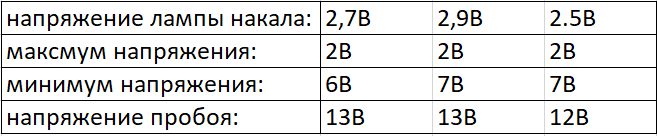
\includegraphics[width=0.7\linewidth]{images/table_1.png}
\caption{Измерения в динамическом режиме}
\label{table_1}
\end{figure}

Здесь минимум напряжения это $E_2$, а максимум это $E_1$ - формула (4). Погрешность измерения в динамическом режиме: $\sigma_E = 0,5$ В.

\item По результатам измерений расчитаем размер электронной оболочки атома инертного газа, заполняющего лампы используя формулы (1 - 3). Эффективную глубину потенциальной ямы $U_0$ можно оценить по формуле (4). Запишем получившиеся значения в таблицу.

\begin{center}
\begin{tabular}{|c|c|c|c|c|}
\hline 
$U_{\text{накала}}$ & $U_0$, эВ & $\sigma_{U_0}$, эВ  & $l,$ пм & $\sigma_l,$ пм\\ 
\hline 
2,5 & 2,00 & 0,53 & 307 & 81 \\ 
\hline 
2,7 & 1,20 & 0,32 & 343 & 91\\ 
\hline 
2,9 & 2,00 & 0,53 & 307 & 81\\ 
\hline 
\end{tabular} 
\end{center}

Итоговое значение для глубины ямы: $U_0 = 1,73 \pm 0,46$ эВ. Для размера электронной оболочки: $l = 319 \pm 84$ пм. Табличные значения для $l = 280$ пм, $U_0 = 2,5$ эВ. В итоге получаем, что размер электронной оболочки совпадает с табличным с учетом погрешности, а глубина ямы нет.

\item По напряжени пробоя понимаем, что газ находящийся в лампе является ксеноном($U_{ion} = 12,1$ эВ).

\end{enumerate}

\subsection{Статический метод}

\begin{enumerate}

\item Проведем измерения для статического метода на тех же напряжениях. Запишем результаты измерений в таблицу:

\begin{figure}[h!]
\centering
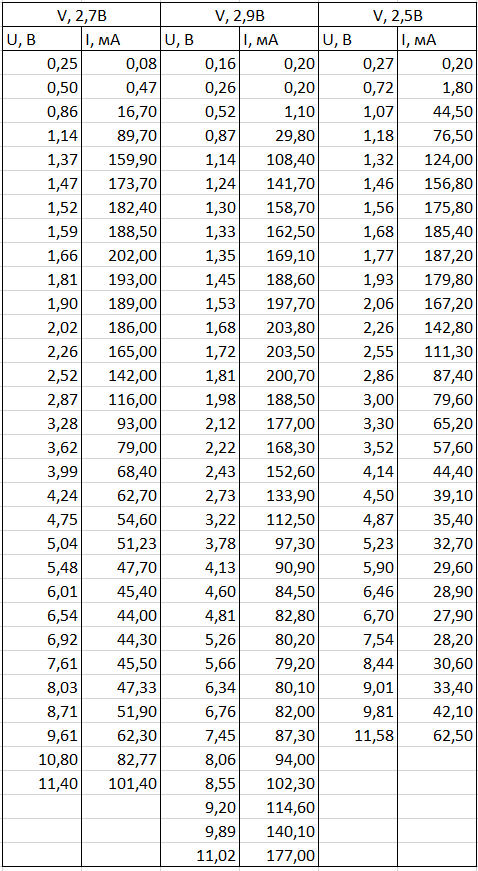
\includegraphics[width=0.7\linewidth]{images/table_2.png}
\caption{Измерения в статическом режиме}
\label{table_2}
\end{figure}

\item Нанесем получившиеся точки на график:

\begin{figure}[h!]
\centering
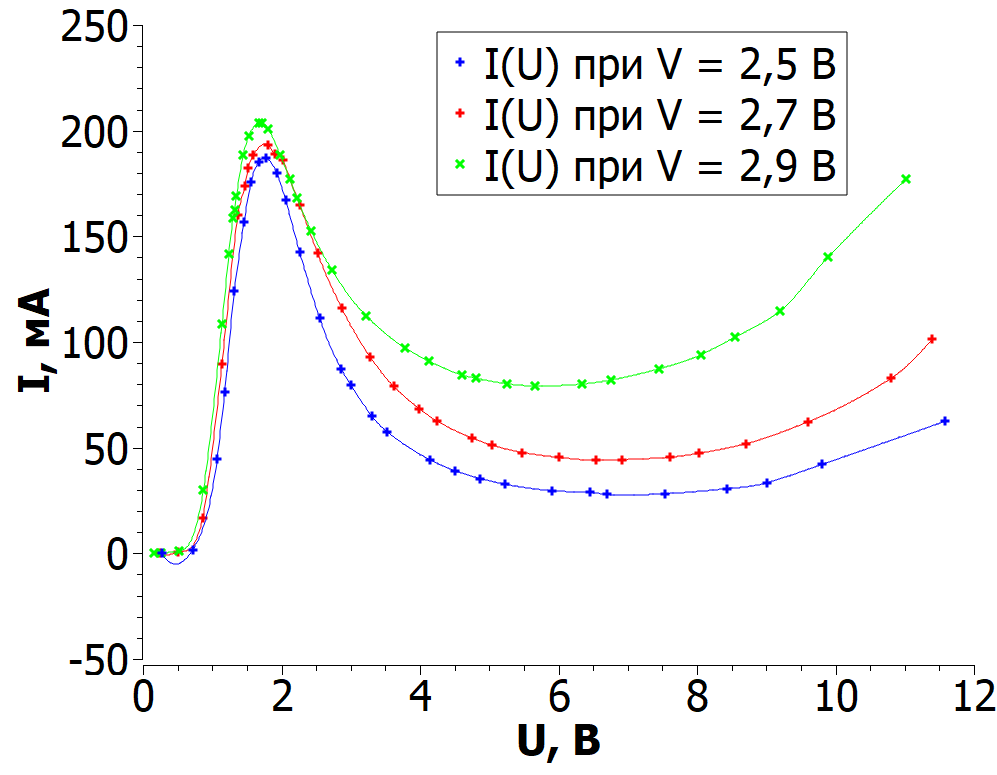
\includegraphics[width = 0.9\linewidth]{images/graph.png}
\caption{График зависимости I(U) в статическом режиме}
\label{graph}
\end{figure}

\item Аналогично расчетам в динамическом режиме приведем расчеты в статическом режиме:

\begin{center}
\begin{tabular}{|c|c|c|c|}
\hline 
$U_{\text{накала}}$, В & 2,5 & 2,7 & 2,9  \\ 
\hline 
$U_{max}$,В & 1,8 & 1,8 & 1,7 \\ 
\hline 
$U_{min}$, В & 6,7 & 6,5 & 5,7 \\ 
\hline 
\end{tabular} 
\end{center}

\begin{center}
\begin{tabular}{|c|c|c|c|c|}
\hline 
$U_{\text{накала}}$ & $U_0$, эВ & $\sigma_{U_0}$, эВ  & $l,$ пм & $\sigma_l,$ пм\\ 
\hline 
2,5 & 2,12 & 0,01 & 310 & 2 \\ 
\hline 
2,7 & 1,96 & 0,01 & 317 & 2\\ 
\hline 
2,9 & 1,5 & 0,01 & 343 & 2\\ 
\hline 
\end{tabular} 
\end{center}

\item Итоговое значение для глубины ямы: $U_0 = 1,86 \pm 0,01$ В, для размера электронной оболочки атома: $l = 323 \pm 3$ пм. Значения отличаются от табличных.

\item Построим график зависимости вероятности рассения электронов (с точностью до константы) от энергии.

\begin{figure}[h!]
\centering
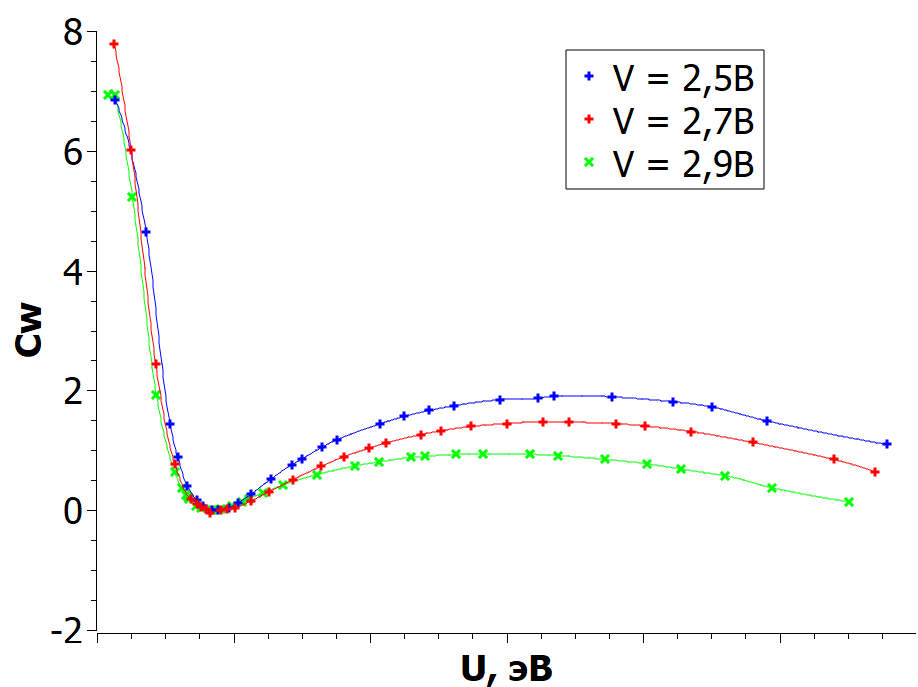
\includegraphics[width = 0.9\linewidth]{images/graph_2.png}
\caption{Зависимость вероятности рассения электронов (с точностью до константы) от энергии}
\label{graph_2}
\end{figure}

\end{enumerate}

\section{Вывод}

Провели измерения для тиратрона. Определили газ, который находится в лампе - ксенон. Получили значения для глуюины ямы в статическом и динамическом методе. В динамическом методе получили совпадение размера электронной оболочки (ввиду большой погрешности, а не высокой точности данных). В статическом методе хоть и была получена высокая точность данных, мы получили значения, отличающиеся от табличных.

\end{document}